%----------------------------------------------------------------------
%                        PROJECT DEFINITION
%----------------------------------------------------------------------
\renewcommand{\projnr}{B4}
\renewcommand{\projtitleshort}{Simulating collisions with SPH}
\renewcommand{\projauth}{Kley}
%
\newcommand{\gsim}{\raisebox{-0.6ex}{$\stackrel{{\displaystyle>}} 
{\sim}$}}
\newcommand{\lsim}{\raisebox{-0.6ex}{$\stackrel{{\displaystyle<}} 
{\sim}$}}
%
\setcounter{section}{0}
\noindent{\normalfont\sffamily\Large\bfseries Project \projnr:  
\projtitleshort}
%
\section{Full title:}
\hspace{1\baselineskip}\\
\centerline{\large ``Simulations of agglomerate collisions with}
\centerline{\large Smooth Particle Hydrodynamics''}
%
\section{General information}\mbox{}
\subsection{Principle investigators:}
\hspace{-\baselineskip}\\\noindent
%
{\bfseries\itshape Kley}, Wilhelm, Prof.~Dr.\\
C4, tenure\\
Date-of-birth: 19. February, 1958, Nationality: German\\
DFG Code number of latest application (KL 650/7-1)\\
Institut f\"ur Astronomie \& Astrophysik\\
Abt.\ Computational Physics\\
Universit\"at T\"ubingen\\
Auf der Morgenstelle 10\\
72076 T\"ubingen\\
Tel: (07071) 29-74007\\
Fax:  (07071) 29-5094\\
Email: wilhelm.kley@uni-tuebingen.de\\
Private address: Herrenbergerstr. 73, 72070 T\"ubingen, Tel.: (07071)  
640085\\
\vspace{1em}\\\noindent
{\bfseries\itshape Speith}, Roland, Dr.\\
Postdoctoral Research Fellow, non-tenure\\
Date-of-birth: 23. June 1966, Nationality: German\\
%% DFG Code number of latest application (if any)\\
Institut f\"ur Astronomie \& Astrophysik\\
Abt.\ Computational Physics\\
Universit\"at T\"ubingen\\
Auf der Morgenstelle 10\\
72076 T\"ubingen\\
Tel: (07071) 29-72043\\
Fax: (07071) 29-5889\\
Email: speith@tat.physik.uni-tuebingen.de\\
Private address: Falkenweg 14, 72076 T\"ubingen, Tel.: (07071) 928073
%%
%%
\subsection{Co-investigators within this Forschergruppe:}
\begin{coilist}
\item J.~Blum (IGEP, TU Braunschweig)
\item C.~P.~Dullemond (MPIA Heidelberg)
\item H.~H.~Klahr (MPIA Heidelberg)
\item G.~Wurm (IfP, Uni M\"unster)
\end{coilist}
%%
%%
\section{Summary (Zusammenfassung)}
%
\subsubsection{Summary:}
%
The initial growth of planetary precursors is accomplished through a
sequence of collisions of small meter-sized agglomerates, so called
pre-planetesimals.  A prerequisite for successful growth is a high sticking
probability of the particles after colliding with each other.  For solid
bodies of cm size or larger the typical collision velocities in
protoplanetary disks are in the range of around 1~m/s up to $>50$~m/s,
depending on the size ratio and the form factor of the bodies. Numerical
simulations show that growth by collisions of {\it rocky} bodies under these
conditions is rather unlikely, and erosion is the primary outcome.  However,
recent experiments indicate that pre-planetesimals consist of {\it porous}
macroscopic dust agglomerates rather than solid rocky bodies which behave
very differently from solid bodies in collisions.  In this project, a
comprehensive survey of three dimensional numerical simulations of
collisions between dust agglomerates will be performed using porosity models
which are calibrated by experimental data from dust experiments.
%
\subsubsection{Zusammenfassung:}
% here the summary in german asa the summary is done
Das anf\"angliche Wachstum der Vorg\"anger von Planeten erfolgt durch eine
Sequenz von Kollisionen von kleinen Meter-gro{\ss}en Agglomeraten, sog.\
Pr\"a-Planetesimalen.  Die wesentliche Voraussetzung f\"ur ein erfolgreiches
Wachstum ist eine gro{\ss}e Haftungswahrscheinlichkeit der Teilchen bei
Kollisionen.  Die typischen Kollisionsgeschwindigkeiten in einer
protoplanetaren Scheibe betragen f\"ur feste K\"orper mit einer Ausdehnung
im cm-Bereich oder gr\"o{\ss}er etwa 1~m/s bis zu $>50$~m/s, je nach
Gr\"o{\ss}enverh\"altnis oder Form der K\"orper.  Numerische Rechungen
zeigen, dass Wachstum bei Kollisionen von {\it steinigen} K\"orpern unter
diesen Bedingungen recht unwahrscheinlich ist und statt dessen die Erosion
\"uberwiegt. Neue Experimente zeigen jedoch, dass Pr\"a-Planetesimale 
aus {\it por\"osen} makroskopischen Staubagglomeraten bestehen, anstatt aus
festen Gesteinsbrocken.  Diese verhalten sich somit bei St\"o{\ss}en
g\"anzlich unterschiedlich.  In diesem Projekt soll unter Verwendung von
dreidimensionalen Simulations\-rechungen ein ausf\"uhrlicher \"Uberblick
\"uber das Verhalten von por\"osen Staubagglomeraten bei Kollisionen
miteinander gewonnen werden.  Dabei werden die notwendigen
Porosit\"atsmodelle anhand experimenteller Daten von Staub-Experimenten
kalibriert.
%
\section{State of the art (Stand der Forschung)}
\subsection{Formation of planetesimals}
The terrestrial planets and the cores of the giant planets (if they have
cores) have been formed from micron sized dust grains through a sequence of
sticking collisions. This requires a growth of over 13 orders of magnitude
in size and more than 40 orders of magnitude in mass.  Recent HST
observations of protostellar disks in Orion at different wavelengths have
been interpreted as evidence for initial grain growth in such disks
({Shuping} {et~al.} 2003).  The growth of planetesimals from micron sized
dust grains to typical sizes of about $10$~km has to be accomplished on time
scales smaller than $\lsim 10$~Myr, due to the limited lifetime of
protoplanetary disks.

In principle, the formation of terrestrial planets and the cores of the
giant planets can be divided into three different stages, which can be
characterized by the type of interaction between the gas and the dust in the
disk. In the {\it first phase}, the dust immersed in the accretion disk
settles towards the midplane of the disk, and they will grow to cm
size. During this process, the dust grains are strongly coupled to the gas
and the orbital velocity of the dust grains equals the orbital velocity of
the gas (Weidenschilling 1980). In the {\it second phase} which includes the
growth from meter sized objects (pre-planetesimals) to planetesimals
(km-sized), the pre-planetesimals are not strongly coupled to the gas and
have larger orbital velocities. They experience a gas drag and lose angular
momentum which leads to a fast radial migration (of the order of 1000~years
per AU for an initial distance of 1~AU from the protostar, see e.g.\
Weidenschilling 1977). This induces two major problems: Firstly, the
pre-planetesimals are the fastest drifters and require a very fast growth
rate, otherwise they get lost to the protostar. Secondly, the
pre-planetesimals have the fastest collision velocities and, as noted by
Benz (2000), rocky-like pre-planetesimals do not tend to stick even for low
velocity collisions.  Moreover, these objects are rather disrupted or
shattered during collisions and no net growth can be observed in these
simulations. The {\it third and last phase} includes the growth from
planetesimals to terrestrial planets. The planetesimals are hardly coupled
to the gas and the relevant interaction is the gravitational attraction
between the planetesimals. Inelastic collisions between the planetesimals
lead to the formation of terrestrial planets on timescales of $10^{7}$ to
$10^{8}$~years (Inaba et al.~2001).

Recent observations of comets and the Deep Impact mission
%% and the observations of near earth asteroids by the NEAR mission
indicate that the first meter
sized objects in the protoplanetary disks have been porous agglomerates and
not brittle materials. Also, laboratory experiments and simulations of dust
growth result in rather fluffy and porous objects (Blum \& Schr\"apler 2004,
Kempf 1999).  Additionally, porous dust grains may explain some extinction
and absorption features in protostellar disks (Voshchinnikov et al.~2006).
Hence, the second growth phase of the planet formation process may primarily
be dominated by the collisions between porous bodies which finally
agglomerate to form planetesimals.

The growth from pre-planetesimals to objects with diameters of about
100~m through a sequence of collisions still presents one of the major
problems in the current theory of planet formation. To investigate this
problem constitutes the main topic of this project.
%
\subsection{Modeling of Collisions}
%
The collisions between planetesimals have been modeled using the Lagrangian
particle method Smooth Particle Hydrodynamics (SPH), that has been
originally developed for the simulation of hydrodynamical problems by
Gingold \& Monaghan (1977) and Lucy (1977). It has been extended to the
simulation of elastic and plastic materials in the beginning of the nineties
in Los Alamos, mainly for simulations with military purposes (see
e.g.~Randles \& Libersky 1996).  By the use of a dynamical fracture model by
Grady \& Kipp (1980), Benz and Asphaug have successfully modeled collisions
between brittle materials (Benz \& Asphaug 1994, 1995, 1999). As noted
above, they do not find a possible growth mechanism by collisions for
pre-planetesimals under the assumption of rocky-like materials (Benz
2000). The essential ingredients for a realistic model include an equation
of state and a model for crack formation in the solid body. For
high-velocity impacts and collisions between brittle materials, the
Tillotson equation of state is very successful as it covers a wide regime of
physical conditions (Tillotson 1962). Physically, fracture is related to the
failure of atomic or molecular bonds. If an applied force acting on a
material is large enough to break the atomic bonds, the material will
fracture and develop cracks. The model of Grady and Kipp is based on two
assumptions: Firstly, brittle materials contain flaws which are sources of
weakness leading to the activation and growth of cracks under tensile
loading. Secondly, the dynamic fracture depends on the rate of tensile
loading, which means, that brittle material that is pulled apart slowly will
develop fewer cracks than a brittle material that undergoes higher strain
rates.

As outlined above, the critical phase in planet formation may be
characterized by collisions between {\it porous} agglomerates, which behave
during collisions completely different from brittle materials.  One major
difference is the dynamical response of grain agglomerates: Normally, for
brittle materials, the strength increases with the strain rate and is
constant for low strain rates. The Grady and Kipp model reproduces this
behavior and yields smaller fragment sizes for higher strain rates. However,
as it is found experimentally, porous agglomerates show different behavior
(Schweiger \& Zimmermann 1999, Iveson et al.~2002). A simple damage model
for porous agglomerates is used in SPH simulations by Sirono (2004): As soon
as the agglomerate reaches either its tensile or compressive or shear
strength, fracture sets in and cracks grow according to the standard damage
evolution equation of the Grady and Kipp model.  The damage model by Sirono
additionally includes a damage restoration effect, through reconnection of
atomic bonds during plastic deformation, the value of damage may
decrease. However, Sirono's model is very limited and requires more physical
considerations for improvements.  Sirono uses a special equation of state
for porous agglomerates which is based on the Murnaghan equation of state
and reads
%
\begin{equation} p(\varrho) = \left\{ \begin{array}{ll}
K(\varrho_0')(\varrho/\varrho_0'-1) & \varrho_0' < \varrho \le
\varrho_\mathrm{c}, \\ \Sigma(\varrho) & \varrho > \varrho_\mathrm{c},
\end{array} \right.  \end{equation}
%
where $\varrho_0'$ is the reference density of an aggregate at no
external stresses. The critical density $\varrho_\mathrm{c}$ is a
function of the reference density $\varrho_0'$. The pressure reaches the
compressive strength as soon as the density $\varrho$ exceeds the
critical density. As soon as the pressure decreases, the behavior of
the agglomerate is again elastic with a different bulk modulus
$K(\varrho_0')$. The influence of porosity is mainly captured in the
dependence of the elastic/plastic material parameters: The bulk modulus
varies as $K(\varrho_0') = K_0 \varphi^\gamma$, where $\varphi$ denotes
the relative density and the exponent $\gamma$ is determined by
measurements (Kendall et al.~1987). Similarly, the compressive
strength, the shear strength and the tensile strength follow power laws.
The dependencies used by Sirono (2004), however, have been based on
measurements of the dynamic behavior of toner particles for different
volume filling factors. Blum \& Schr\"apler (2004) find a significant
weaker dependence of the shear strength on the porosity than implied be the
Sirono model, which might lead to different results concerning the sticking
efficiency. Other promising models that consider porosity in impact
simulations are currently developed in the community: Jutzi (2004) has
adopted the P-$\alpha$ model by Herrmann (1969) in an existing SPH code,
and W{\"u}nnemann et~al.\ (2006) have recently presented a new
strain-based porosity model for the use in hydrocode simulations (the
$\varepsilon$-$\alpha$ model). 

%
\section{Preliminary work (Eigene Vorarbeiten)}
%
The applicants have been working on the field of planet formation and the
physics of accretion disks for several years.  We have performed many
numerical simulations of accretion disks, with emphasis on accretion disks
in cataclysmic variables and protostellar accretions disks (e.g.\ Kley \&
Lin 1996, 1999; Kunze et al.\ 2001; Speith \& Kley 2003; G\"unther et al.\
2004).  The dynamical interaction of a young protoplanet with its
surrounding protoplanetary disk has been studied in great detail by the
applicants using either grid- or particle-based numerical methods (e.g.\
Kley 1999; D'Angelo et al.\ 2003; Kley et al.\ 2004; Kley \& Dirksen 2006;
de Val-Borro et al.\ 2006; Sch\"afer et al.~2004b; Sch\"afer 2005 and
references therein).
%

The numerical particle method Smooth Particle Hydrodynamics (SPH) has been
widely applied to different astrophysical problems within our research group
(e.g.\ Kunze et al.\ 2001; Kunze \& Speith 2005).  Additionally, the
technical issues of the method have been studied in detail and improved
(e.g.\ Speith 1998; Speith \& Kley 2003).  By the use of a new artificial
bulk viscosity, the migration of protoplanets in a protoplanetary accretion
disk has been studied successfully (Sch\"afer et al.~2004b). Efficient
(parallel) SPH codes have been developed in close collaboration with
computer scientists as part of the Sonderforschungsbereich SFB 382
``Verfahren und Algorithmen zur Simulation physikalischer Prozesse auf
H\"ochstleistungsrechnern'' (Ganzenm\"uller et al.~2003; Hipp et al.~2004).
%

Following the approach by Benz and Asphaug (1994), the SPH code {\tt
ParaSPH} has been extended by C.~Sch\"afer for the simulation of
elasto-plastic, ductile and brittle materials (Sch\"afer 2005). The code
{\tt ParaSPH} (first designed by M.~Hipp in T\"ubingen within the SFB 382)
runs now on various computer architectures, including shared and distributed
memory parallel supercomputers. By the use of hybrid-parallel programming,
that is the combination of both OpenMP directives and instructions, and the
use of a Message Passing Interface (MPI) implementation, {\tt ParaSPH}
performs and scales excellently.

The code has been tested using standard tests, such as the collision of two
perfectly elastic rings. The damage model which is based on the ansatz by
Grady and Kipp has been successfully compared to theoretical values for the
simulation of a brittle rod under tension. Additionally, the code has
accurately reproduced the results of the laboratory high-velocity impact
experiment by Ahrens \& Rubin (1993). The code allows for the choice between
several equations of state, such as the Murnaghan equation of state, in
which the pressure depends non-linearly on the density, and the Tillotson
equation of state that additionally includes the dependence on the change of
internal energy.  For details on code related issues, see Sch\"afer (2005),
and first results are presented in Sch\"afer et al.~(2004a).

Finally, the approach by Sirono (2004) which is described in the previous
section has been included in the {\tt ParaSPH} code and the simulations
performed by Sirono (2004) have been improved by the use of higher
resolutions (Sch\"afer 2005). The results of the collisions between porous
agglomerates are very promising: While brittle meter sized objects fragment
during collisions with relative velocities in the range between 10-20~m/s,
porous ice agglomerates tend to deform plastically and are not disrupted
even for collision speeds of 30~m/s. However, this has been so far only
shown for a fixed size ratio of 1/3 of the target to the impactor and only
for ice agglomerates. Recent calculations (Sch\"afer et al.~in prep.)
indicate that equal sized bodies might also tend to fragment since the
sticking efficiency strongly depends on the size ratio of the colliding
bodies. Additionally, the target body mainly changes its shape during the
collision rather than being compacted efficiently. Fig.~\ref{fig:b4_1} shows
the impact of a smaller porous pre-planetesimal into a larger one for
typical conditions within a protoplanetary disk.

\begin{figure}
\centering{
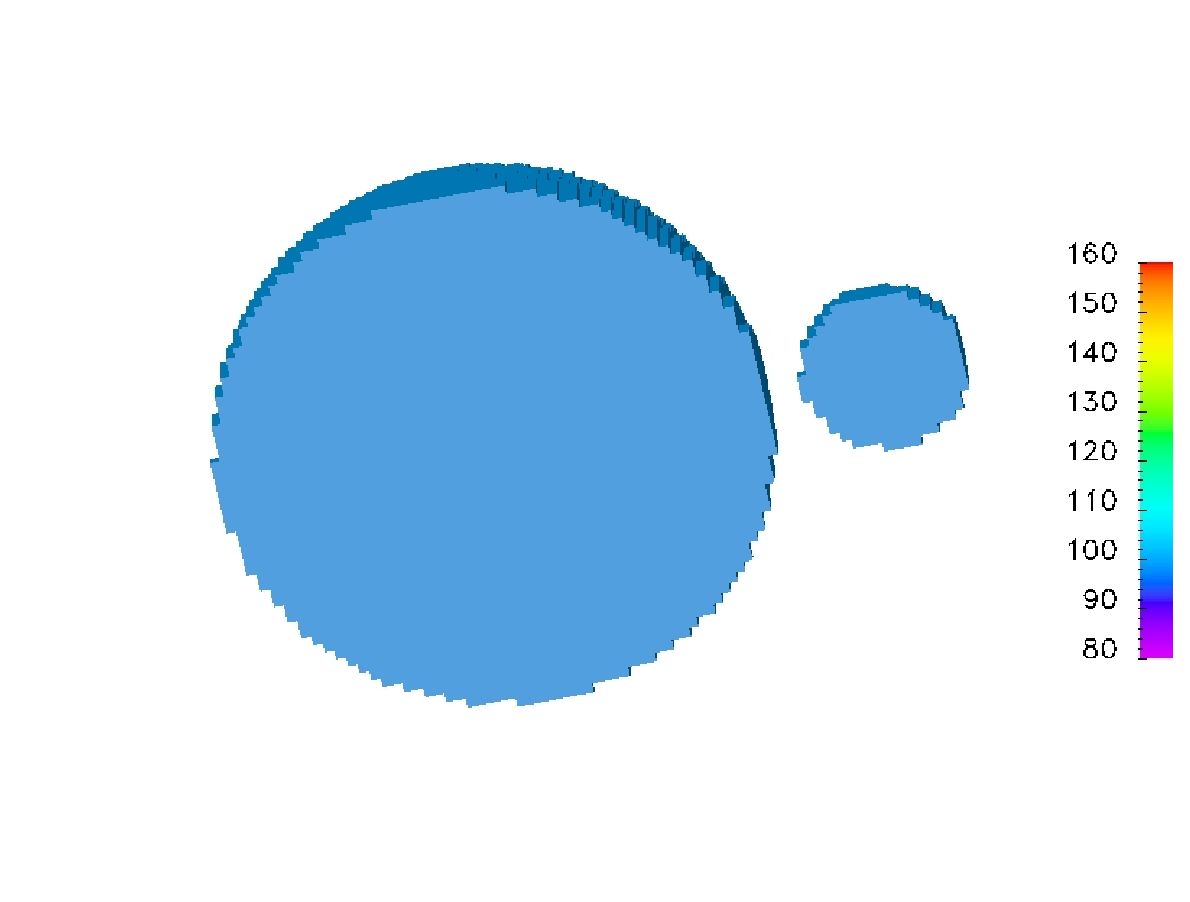
\includegraphics[scale=0.6]{b4fig1.eps}\\
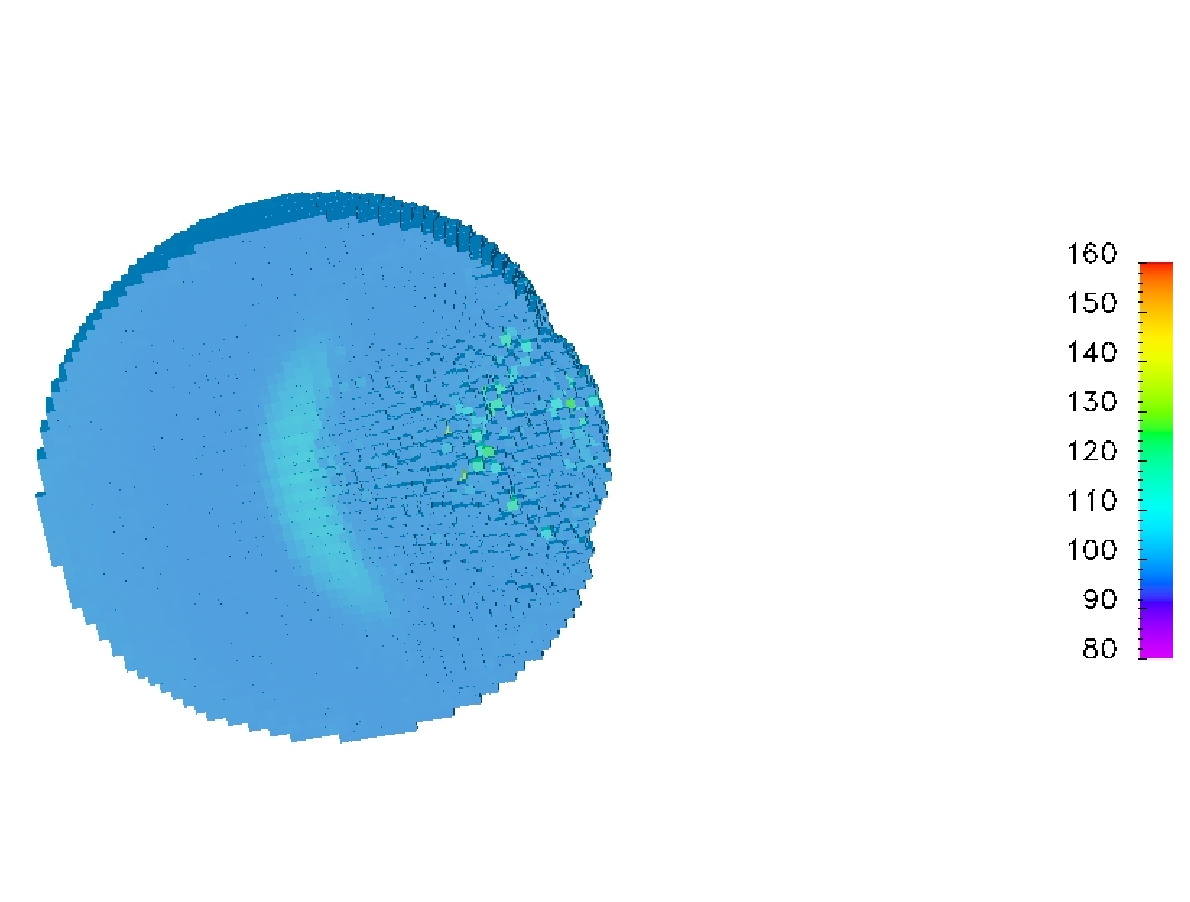
\includegraphics[scale=0.6]{b4fig2.eps} }
\caption{Simulation of an
impact: A smaller ice agglomerate impacts into a larger porous body with an
initial speed of 20~m/s. The radii of the agglomerates are 1~m and 30~cm,
respectively. The color code shows the density in units of kg/m$^3$, the
initial porosity is 0.9. In contrast to collisions between solid brittle
materials, where the impactor gets disrupted, the impacting body can enter
the target and is incorporated into it. The porosities of the target and the
impactor hardly change, and the impactor deforms plastically.}
\label{fig:b4_1}
\end{figure}
%
%
% Here follows the own refereed publications by the PIs in relation to
% the project proposed here.
%
\ownpubltitle{Own publications related to the Forschergruppe:}
%
% BELOW IS ONLY AN EXAMPLE OF TWO ENTRIES. SEE THE ADDITIONAL FILES SENT
% TO YOU WITH ALL THE REFERENCES FROM THE VORANTRAG
%
\begin{ownpubl}
\item {D'Angelo}, G., {Kley}, W. \& {Henning}, T. (2003)
   Orbital Migration and Mass Accretion of Protoplanets in
   Three-dimensional Global Computations with Nested Grids
   \apj, \textbf{586}, 540
\item de Val-Borro, M., Edgar, R.G., Artymowicz, P., Ciecielag, P.,
   Cresswell, P., D'Angelo, G., Delgado-Donate, E.J., Dirksen, G.,
   Fromang, S., Gawryszczak, A., Klahr, H., Kley, W., Lyra, W., Masset,
   F., Mellema, G., Nelson, R., Paardekooper, S.-J., Peplinski, A.,
   Pierens, A., Plewa, T., Rice, K., Sch\"afer, C., Speith, R.\ (2006)
   A comparative study of disc-planet interaction, \mn, in press
\item Ganzenm\"uller, S., Hipp, H., Kunze, S.,
Pinkenburg, S., Ritt, M., Rosenstiel, W., Ruder, H. and Sch\"afer,
C.\ (2003) Efficient and Object-Oriented Libraries for Particle Simulations, in:
\textit{High Performance Computing in Science and Engineering '03}
\item G\"unther, R., Sch\"afer, C., Kley, W.\ (2004)
   Evolution of irradiated circumbinary disks
   \aap, \textbf{423}, 559
\item Hipp, M., Pinkenburg, S., Holtwick, S., Kunze, S., Sch\"afer, C.,
Rosenstiel, W., and Ruder, H.\ (2004) Libraries and Methods for Parallel
Particle Simulations, in: \textit{High Performance Computing in Science
and Engineering '04}
\item Kley, W. \& Dirksen, G. (2006)
   Disk eccentricity and embedded planets
   \aap, \textbf{447}, 369
\item Kley, W. \& Lin, D.N.C. (1996)
   The Structure of the Boundary Layer in Protostellar Disks
   \apj, \textbf{461}, 933
\item Kley, W. \& Lin, D.N.C. (1999)
   Evolution of FU Orionis Outbursts in Protostellar Disks
   \apj, \textbf{518}, 833
\item Kley, W., {Peitz}, J. \& {Bryden}, G. (2004)
   Evolution of planetary systems in resonance
   \aap, \textbf{414}, 735
\item Kunze, S., Speith, R.~and Hessman,
F.~V.~(2001) Substantial stream-disc overflow found in three-dimensional
SPH simulations of cataclysmic variables, \mn, \textbf{322}, 499
\item Kunze, S. \& Speith. R. (2005)
   SPH Simulations of the 2:1 Resonance in Accretion Disks,
   in: \textit{The astrophysics of cataclysmic variables and related
     objects}, ASP Conf.\ Ser., {\bf 330}, 389
\item Sch{\"a}fer, C., Speith, R., G{\"u}nther, R., \& Kley, W.\ (2004a)
   Impact Simulations with SPH,
   Astronomische Nachrichten Supplement, {\bf 325}, 84
\item
Sch\"afer, C., Speith, R., Hipp, M.~and Kley, W.\ (2004b) Simulations of
planet-disc interactions using Smoothed Particle Hydrodynamics, \aap,
\textbf{418}, 325
\item Sch\"afer, C.~(2005) Application of Smooth
Particle Hydrodynamics to selected Aspects of Planet Formation, PhD
thesis, Eberhard-Karls-Universit\"at T\"ubingen
\item Speith, R.~(1998) Untersuchung von Smoothed Particle
   Hydrodynamics anhand astrophysikalischer Beispiele, PhD
thesis, Eberhard-Karls-Universit\"at T\"ubingen
\item Speith, R.~and Kley, W.~(2003) Stability of the viscously spreading ring, \aap,
\textbf{399}, 395
\end{ownpubl}
%
%
\section{Goals (Ziele)}
%

The primary goal of this project is to understand the growth of medium sized
pre-planetesimals through collisional aggregation.  For this purpose we will
use numerical models to investigate the outcome of collisions between
macroscopic dust agglomerates.  Detailed comparison between our models and
the laboratory experiments in projects \projwurm\ and \projblumtrie\ for
small ($<$ dm) agglomerates will allow both, the testing of the numerical
algorithms, as well as a deeper understanding of the phenomena observed in
the laboratory.  In the following, emphasis will be put on collisions
between particles with sizes which are too big to be used in the laboratory.
We will perform three dimensional simulations of collisions between porous
pre-planetesimals in order to study possible growth mechanisms and derive
the sticking efficiencies for various size ratios, porosities, particle
materials, and relative velocities.

\noindent
The following challenges have to be met:
%
\begin{itemize}
\item Development of a realistic model for the elastic and plastic
behavior of porous agglomerates.
\item Validation of the code by comparing the simulation results to  
the outcome of experiments.
\item Determination of the mass distribution of fragments after
collisions and the catastrophic disruption thresholds for
pre-planetesimals.
\item Study of subsequent impacts on one porous agglomerate.
\item Determination of the dust production by pre-planetesimal  
collisions.
%and possible influences on the extinction and absorption of
%protoplanetary disks.
\end{itemize}


\section{Work schedule (Arbeitsprogramm)}
%
\subsection{Methods}
%
%
The existing code will firstly be adapted to model the results of the recent
impact experiments by Wurm et al.~(2005a,b), Langkowski \& Blum (in prep.),
and Teiser \& Blum (in prep.). The Sirono model requires the knowledge of
the dependencies of the material parameters (such as the bulk and shear
moduli, the tensile, compressive and shear strengths) on the porosity. These
dependencies have been derived for ice agglomerates by Sirono~(2004). In the
case of dust agglomerates, the material parameters for some specific
porosities can be extracted from the experiments presented in Wurm et
al.~(2005a,b), Blum \& Schr\"apler~(2004), Langkowski \& Blum (in prep.),
and Teiser \& Blum (in prep.). We will fit their data to obtain the shear,
compressive and tensile strengths and the elastic properties of the dust
agglomerates for all filling factors or porosities, respectively. The best
fit data will be used to model the impact experiments by Wurm et
al.~(2005a,b), Langkowski \& Blum (in prep.) and Teiser \& Blum (in prep.),
and to compare the fragment sizes of the ejecta and the impact crater
radii. Then, the fitted values will be modified such that the results of the
simulation resemble the experimental outcome.  In this way we will acquire a
calibrated Sirono model for dust agglomerates.  In order to use a more
realistic equation of state and allow for a non-linear dependence of the
pressure on the density, the Sirono model has to be extended.

With the final (i.e.\ calibrated) code version, we intend to focus on
two-body collisions. The parameter space for the collisions between two
pre-planetesimals is tremendously wide: Size ratio of the pre-planetesimals,
collision velocity, impact angle, initial porosity, elastic and plastic
material parameters (compressive, tensile and shear strength, bulk and shear
modulus) need to be varied in order to obtain reliable statistics and cover
the uncertainties in the knowledge about the material properties of
pre-planetesimals.

The whole survey of collisions will then allow us to predict the collisional
outcome between two agglomerates with specified parameters.  The goal is to
provide, in analogy to Benz \& Asphaug (1999), the catastrophic disruption
coefficients which are basic input parameters in statistical simulations
dealing with the dust growth in the whole disk, such as coagulation
simulations of dust growth or the modeling of planetary accretion, that is
the growth from planetesimals to protoplanets and terrestrial planets (see
e.g.~Weidenschilling 2000; Dullemond \& Dominik 2004; Inaba et
al.~2001). The catastrophic disruption coefficient is the kinetic energy in
the collision divided by the target mass
%
\begin{equation} Q_\mathrm{D}= \frac{1}{2}mv^2/M, \end{equation}
%
when the collision leads to the complete disruption of the target, and
the mass of the largest remaining fragment is half the target mass.

The mass distribution of the fragments after a collision can be determined
by the complete analysis of the collisional remnants.  This is essential
input to the coagulation/fragmentation project \projdul{}, and via such
models will affect the model predictions for IR spectra of the
protoplanetary accretion disk in conjunction with project \projwolf{}.
% An important goal of
% the project will be to derive observable influences of material properties
% of the pre-planetesimals on the IR spectra of the protoplanetary accretion
% disk in conjunction with project \projwolf. 
% This can be achieved if the
% complete mass spectra of the fragments after the collision is determined and
% the production of dust grains from larger objects is known. The re-formed
% dust grains in the $\mu$m size change the IR spectra significantly. The
% results of the simulations can therefore be compared to observations of the
% SPITZER telescope (Bryden et al.~2006).
%
%----------------------------------------
\subsection{Schedule}
%
\subsubsection{First year}
%
%
Development of a realistic model for the elastic and plastic behavior of
porous agglomerates: Extension of the Sirono model and calibration of the
code. This part of the project will be tackled in very close collaboration
with J.~Blum and G.~Wurm (cf.\ Project B1-B3).  We will first use data from
their experiments as published in Blum \& Schr\"apler~(2004), Wurm et al.\
(2005a,b), Langkowski \& Blum (in prep.), and Teiser \& Blum (in prep.)  to
obtain a realistic model for the elastic properties and compressive, tensile
and shear strengths for dust agglomerates.

Dedicated impact experiments for the deduction of elastic flattening,
plasticity, onset of fragmentation and fragment mass distribution for
dust agglomerates of various sizes and porosities will be carried out
in the Braunschweig and M\"unster laboratories.

When the code will successfully reproduce the experimental
outcome, the simulations will be extended into a larger size range which
cannot be examined in the laboratory.

\subsubsection{Second year}

Determination of the catastrophic disruption thresholds for
pre-planetesimals: The main task of the project requires an immense
number of simulations in order to achieve reliable statistics.
Therefore, the setup of the simulations and the analysis of the results
have to be automated. We plan simulations involving bodies of sizes
ranging between 1~cm and 100~m.
At first, we will focus on one target and impactor material and vary
only the porosity of the target and the kinetic energy of the collision,
while all other material parameters are kept fixed, and we will focus on
collision velocities that are predicted by \projklahr. In this way, the
{\it catastrophic disruption threshold} $Q_\mathrm{D}$ can be determined
as a function of the target size and the initial porosity.  To study the
differences in oblique impacts, some of the simulations will be repeated
using different angles (e.g.\ 30 and 60 degrees) of incidence.

Study of subsequent collisions: The code will 
additionally be used to simulate the experiments which are performed in
\projwurm, that is the evolution of a large dusty body under the
influence of multiple impacts. In this way, the numerical model will be
improved continuously with more data becoming available.

\subsubsection{Third year}
%
%
Determination of the mass distribution of fragments after collisions:
The simulations demand for high
resolutions in order to resolve the fragments on the lower length scale.
The automated analysis of the simulation results includes the detection
of the fragments, their mass, momentum and angular momentum.
Accordingly, the remains of the target, especially the changes in the
form factor/shape and the porosity are recorded. The results from these
simulations will be important for the dust coagulation project \projdul\
as they provide necessary input for the coagulation equations.

Determination of the dust production by pre-planetesimal collisions:
The collisions with the most likely parameters
will be simulated at very high resolutions to investigate the dust
production by collisions between larger objects. However, it will be not
possible to resolve the fragments in the micron size range if the
initial agglomerates are meter-sized. The production of particles in the
micron size range can be predicted by the scaling of the mass
distribution of the fragments to lower sizes, though.

\subsection{Literature}
%
% Here follows a general literature list related to the topic of the
% proposal, just like a literature list for a scientific paper.
%
% AGAIN ONLY EXAMPLES ARE LISTED NOW
%
\begin{literature}
\item Ahrens, T.~J.\ and Rubin, A.~M.\ (1993) Impact-induced tensional
failure in rock, \jgr, \textbf{98}, 1185
\item Beckwith, S.~V.~W.~and Sargent, A.~I.\ (1996) Circumstellar disks
and the search for neighbouring planetary systems, \nat, \textbf{383},
129
\item Benz, W.\ (2000) Low velocity collisions and the Growth of
Planetesimals, \ssr, \textbf{92}, 279
\item Benz, W.~and Asphaug, E.\ (1994) Impact simulations with fracture.
I - Method and tests, \ica, \textbf{107}, 98
\item Benz, W.~and Asphaug, E.\ (1995) Simulations of brittle solids
using Smooth Particle Hydrodynamics, \cpc, \textbf{87}, 253
\item Benz, W.~and Asphaug, E.\ (1999) Catastrophic Disruptions
Revisited, \ica, \textbf{142}, 5
\item Blum, J.\ and Schr\"apler, R.\ (2004) Structure
and Mechanical Properties of High-Porosity Macroscopic Agglomerates
Formed by Random Ballistic Deposition, \prl, \textbf{93}, 115503
\item Blum, J.\ (2004) Grain Growth and Coagulation, in: \textit 
{Astrophysics
of Dust}, ASP Conference Series, Vol. 309 (Eds. A.~Witt, G.~Clayton and
B.~Draine), 369
\item
{Brice{\~n}o}, C., {Vivas}, A.~K., {Calvet}, N., {et~al.} (2001),
  Science, {\bf 291}, 93
%\item {Bryden}, G., {Beichman}, C.~A., {Trilling}, D.~E., {Rieke},
%G.~H., {Holmes}, E.~K., {Lawler}, S.~M., {Stapelfeldt}, K.~R., {Werner},
%M.~W., {Gautier}, T.~N., {Blaylock}, M., {Gordon}, K.~D., {Stansberry},
%J.~A.~and {Su}, K.~Y.~L.~(2006) Frequency of Debris Disks around
%Solar-Type Stars: First Results from a Spitzer MIPS Survey, {\apj},
\textbf{636},1098
\item
Dullemond, C.~P.\ and Dominik, C.~(2005) Dust coagulation in
protoplanetary disks: A rapid depletion of small grains. \aap,
\textbf{434}, 971
\item Gingold, R.~A.~and Monaghan, J.~J.~(1977) Smoothed Particle
Hydrodynamics: Theory and application to non-spherical stars, \mn,
\textbf{181}, 375
\item Grady, D.~E.~and Kipp, M.~E.~(1980) Continuum Modelling of
explosive fracture in oil shale,
\textit{Int.~J.~Rock~Mech.\ Min.~Sci.~Geomech.~Abstr.}, \textbf{17}, 147
\item Haisch, K.~E., Lada, E.~A.~and Lada, C.~J.~(2001) Disk Frequencies
and Lifetimes in Young Clusters, \apj, \textbf{553}, L153
\item Inaba, S., Tanaka, H., Nakazawa, K., Wetherill, G.~W.~and Kokubo,
E.~(2001) High-Accuracy Statistical Simulation of Planetary Accretion:
II. Comparison with N-Body Simulation, \ica, \textbf{149}, 235
\item Iveson, S.~M., Beathe, J.~A.~and Page, N.~W.~(2002) The dynamic
strength of partially saturated powder compacts: The effect of liquid
properties, \textit{Powder Techn.}, \textbf{127}, 149
\item Jutzi, M. (2004) , Diploma Thesis, University of Bern
\item Kalas, P., Graham, J.~R., Clampin, M.~C.~and Fitzgerald,
M.~P.~(2006), First scattered light images of debris disks around
HD~53143 and HD~139664, \apj, \textbf{637}, L57
\item {Kempf}, S., {Pfalzner}, S.~and {Henning}, T.~K.~(1999)
N-Particle-Simulations of Dust Growth. I. Growth Driven by Brownian
Motion, \ica, \textbf{141}, 388
\item Kendall, K., Alford, N.~McN.~and Birchall, J.~D.~(1987) A new
method for measuring the surface energy of solids, \nat, \textbf{325},
794
\item Lucy, L.~B.~(1977) A numerical approach to the testing of the
fission hypothesis, \apj, \textbf{82}, 10134
\item
{Malfait}, K., {Waelkens}, C., {Waters}, L.~B.~F.~M., {et~al.} (1998),
   \aap, {\bf 332}, L25
\item
{McCaughrean}, M.~J., {Stapelfeldt}, K.~R., \& {Close}, L.~M. (2000),
   Protostars and Planets IV, 485
\item Randles, P.~W.~and Libersky, L.~D.~(1996) Smoothed Particle
Hydrodynamics: Some recent improvements and applications,
\textit{Comp.~Methods~Appl.~Mech.~Engrg.}, \textbf{139}, 375
\item Schweiger, A~and Zimmermann, I.~(1999) A new approach for the
measurement of the tensile strength of powders, \textit{Powder Techn.},
\textbf{101}, 7
\item
{Shuping}, R.~Y., {Bally}, J., {Morris}, M., \& {Throop}, H. (2003),
   \apj, Letters, {\bf 587}, L109
\item Sirono, S.\ (2004) Conditions for collisional growth of a grain
aggregate, \ica, \textbf{167}, 431
\item Tillotson, J.~H.~(1962) Metallic equations of state for
hypervelocity impact, \textit{General Atomic Report GA-3216}
\item Voshchinnikov, V.~B.~Il'in, Henning, T.~and Dubkova, D.~N.\ (2006)
Dust extinction and absorption: The challenge of porous grains, \aap,
\textbf{445}, 167
\item Weidenschilling, S.~J.~(1977) Aerodynamics of solid bodies in the
solar nebula, \mn, \textbf{180}, 57
\item Weidenschilling, S.~J.~(1980) Dust to planetesimals - Settling and
coagulation in the solar nebula, \ica, \textbf{44}, 172
\item Weidenschilling, S.~J.~(2000) Formation of Planetesimals and
Accretion of the Terrestrial Planets, \ssr, \textbf{92}, 311
coagulation in the solar nebula, \ica, \textbf{44}, 172
\item
{Wilner}, D.~J. \& {Lay}, O.~P.~(2000), Protostars and Planets IV, 509
\item Wurm, G., Paraskov, G.~and Krauss, O.~(2005a)
Ejection of dust by elastic waves in collisions between millimeter- and
centimeter-sized dust aggregates at 16.5 to 37.5 m/s impact velocities,
\phre, \textbf{71(2)}, 021304
\item Wurm, G., Paraskov, G.~and Krauss,
O.~(2005b) Growth of planetesimals by impacts at $\sim$25 m/s, \ica,
\textbf{178}, 253
\item W{\"u}nnemann, K., Collins, G.~S., Melosh, H.~J.~(2006) A
strain-based porosity model for use in hydrocode simulations of impacts
and implications for transient crater growth in porous targets, \ica,
\textbf{180}, 514
\end{literature}



\section{External/International collaborations}
\begin{collablist}
%\item[Bern] Collaboration with the research group of Prof.~Dr.~W.~Benz
%from the University of Bern who
%is one of the leading experts in the field of SPH simulations for solid
%bodies.
\item[Nagoya] Collaboration with Dr.~S.~Sirono from the University of
Nagoya who has invented the
model for porous agglomerates that will be used for the simulations.
\item[Freiburg] Collaboration with the research group of  
Dr.~S.~Hiermaier from the
Ernst-Mach-Institut in Freiburg who is one of the leading experts in  
the field
of impact simulations.
\end{collablist}


\section{Link to other projects of the Forschergruppe}
\begin{linkproj}
\item[\projblum{}, \projwurm{} and \projblumtrie{}] The input parameters
for the simulations of the agglomerates,
e.g.~shear and tensile strengths, sound speed and shear and bulk moduli,
and especially their dependencies on the volume filling factors will  
be obtained from the projects
\projblum{}, \projwurm{} and \projblumtrie{}. Especially in the first
year, when the PhD student will calibrate the SPH code using
experimental data, the collaboration will be intensive.
\item[\projklahr{}] Project \projklahr{} provides input on the typical
impact velocities that are expected in a turbulent protoplanetary
accretion disk. Thus, the simulation survey can be restricted on the
relevant case.
\item[\projdul{}] The survey of collisions conducted in
this project includes the determination of the mass distribution of the
fragments and the catastrophic disruption coefficients which are  
needed for the dust coagulation
simulations of project \projdul{}.
% \item[\projwolf{}] The data from high resolution runs will
% give predictions on the regeneration
% of mm-sized dust particles that are observed in the (sub-)millimeter and
% infrared. Hence, the SPH simulations will provide dust production rates
% (together with the data from \projklahr\ that provides collision rates
% and probabilities) that can be used in the radiative transfer model from
% \projwolf.
\end{linkproj}



\section{Team members (Zusammensetzung der Arbeitsgruppe)}
%
% NOTE: Only list non-DFG-funded team members.
% NOTE: Also list technical assistents, students etc involved in the project
%
\begin{teamlist}
% -> Willy, some notes?
\item[Kley, W., Prof.~Dr.~(C4)]\mbox{}\\
Team leader. Supervises the PhD student funded through the project and
provides extensive expertise in computational physics and numerics.
\item[Speith, R., Dr.]\mbox{}\\
Team co-leader. Provides extensive expertise in numerical methods,
especially the Lagrangian particle method Smooth Particle
Hydrodynamics. Has widespread experience in parallel computing for
shared memory architectures using OpenMP directives and distributed
memory architectures with the Message Passing Interface (MPI).
\item[Sch\"afer, C., Dr.]\mbox{}\\
Internal collaborator. Provides extensive knowledge about the
SPH code {\tt ParaSPH} and the simulations of brittle and porous
materials.
\item[Geretshauser, R.]\mbox{}\\
Student collaborator. Code-Testing and parameter studies.
%%%%%%
%%\item[Blum, J., Prof.~Dr.~(C3)]\mbox{}\\
%%Team collaborator. Hosts the PhD student during a visit in Braunschweig
%%where the experimental setups of project \projblumtrie\ will be
%%discussed.
%%In the first year the PhD student strongly relies on the data which was
%%already measured by him and G.~Wurm in order to adopt the Sirono  
%%model to dust
%%agglomerates.
%%Specific, high temporal resolution impact experiments will be
%%performed for the calibration of the SPH code.
%%\item[Dullemond, C.~P., Dr.]\mbox{}\\
%%Team collaborator. Hosts the PhD student during a visit in Heidelberg.
%%Has excellent expertise in numerical solutions of the coagulation  
%%equations.
%%\item[Klahr, H.~H., Dr.]\mbox{}\\
%%Team collaborator. Hosts the PhD student during a visit in Heidelberg.
%%Provides excellent knowledge about the dust dynamics in turbulent
%%protoplanetary accretion disks.
%%\item[Wurm, G., Dr.]\mbox{}\\
%%Team collaborator. Hosts the PhD student during a visit in M\"unster
%%where the experimental setups of project \projwurm\ will be discussed.
%%In the first year the PhD student strongly relies on the data which was
%%already measured by him and J.~Blum in order to adopt the Sirono  
%%model to dust
%%agglomerates.
%%Specific, high temporal resolution impact experiments will be
%%performed for the calibration of the SPH code.
\end{teamlist}
\vspace{1em}



\section{Funding requested}
The following table gives the full overview of requested
funding:\vspace{1\baselineskip}\\
%
% The table that follows is the overview over the full requested
% funding, including the positions, travel, consumables and ``other
% costs'' (which might include transportation costs of radioactive
% material or the rent of a drop tower or such).
%
\centerline{\begin{tabular}{||l|r|r|r||}
\hline \hline & Year 1 & Year 2 & Year 3 \\ \hline %
Personnel (1 PhD-students: E13/2)   & \hfil 24.000 & 24.000 & 24.000 \\
Consumables                        & \hfil - & \hfil - & \hfil - \\
Travel			   	   & \hfil 2.760  & \hfil 2.500 &  \hfil 570\\ \hline
Other costs                        & \hfil 2.000 & \hfil - & \hfil - \\
\hline
{\bf Total:}                       & 28.760  & 26.500  & 24.570  \\
\hline \hline
\end{tabular}
}
\vspace{1em}\\
Below these costs are explained in more detail:

\subsection{Personnel (Personalbedarf)}
\begin{teamlist}
\item[PhD-Student 1 (E13/2)]\mbox{}\\
The PhD student will extend the porosity model and include  
experimentally
measured coefficients into the model. He/she will then perform detailed
parameter studies to determine the outcome of collision simulations.
\end{teamlist}

\subsection{Consumables (Verbrauchsmaterial)}

none

\subsection{Travel expenses in addition to Project Z (Reisekosten)}
%
% Here only travel expenses not related to usual regular Forschergruppe
% meetings and the overall per capita budget for conferences.
%
In the first year during the calibration of the model, the PhD student has
to visit Braunschweig and M\"unster for two weeks each in order to discuss
the model with J.~Blum and G.~Wurm and to participate in the experiments.
In the second year, two shorter meetings (1 week) at Braunschweig and
M\"unster are required to discuss the results of the simulations with larger
objects that are not feasible in the laboratory.  Also, the PhD student will
visit Heidelberg for two weeks for the collaboration with projects
\projklahr{}, \projdul{}. In the last year, the PhD student will
visit Heidelberg for one week to discuss the result of the simulations.

The travel costs by train to Braunschweig, Heidelberg and
M\"unster are 180~EUR, 70~EUR and 180~EUR, respectively. 
The per diem cost for food and lodging is estimated as 100 EUR per day.

Estimated costs in EUR per year:\vspace{1\baselineskip}\\
%
%
\centerline{
\begin{tabular}{||l|r|r|r||}  \hline
\hline         & Year 1   & Year 2 & Year 3 \\ \hline %
Braunschweig   &  1.380  &   680     & -    \\ \hline
Heidelberg     & -       & 1.140     &  570 \\ \hline
M\"unster      &  1.380  &   680     & -    \\
\hline \hline
{\bf Total:}   &  2.760  & 2.500     &  570 \\ \hline \hline
\end{tabular}}
%\centerline{
%\begin{tabular}{||l|l|l|l||}  \hline
%\hline         & Year 1   & Year 2 & Year 3 \\ \hline %
%%Bern           &  250  & -         &  -     \\ \hline
%Braunschweig   &  680  &  480      & -      \\ \hline
%Heidelberg     & -     & 1.140      &  570    \\ \hline
%M\"unster      &  680  &  480      &       - \\
%\hline \hline
%{\bf Total:}   & 1.360 & 2.100    &  570 \\ \hline \hline
%\end{tabular}}

\subsection{Other costs (Sonstige Kosten)}
The PhD student requires a mobile personal computer (laptop) to work
and to present his results during the visits in Braunschweig,
Heidelberg and M\"unster. The cost for this laptop (MacBook Pro) will be
approximately EUR 2000.

\section{Preconditions for carrying out the project at home institution}
%
% This is one of the main subsections of a DFG Normalverfaren proposal.
% Several of the subsubsections in this subsection we have placed in  
%their
% own subsections above (like team members, collaborations). What  
%remains
% are the following three subsections. For those not familiar with  
%these,
% we refer to the DFG Merkblatt on Normalverfahren-proposals.
%
\subsection{Scientific equipment available (Apparative Ausstattung)}
%
% Please list those larger instrument available to you for the  
%project (if
% applicable also larger computer equipment in case you need substantial
% amounts of computer time).
%
In additions to numerous individual workstations at the Institut f\"ur
Astronomie und Astrophysik, we have the following computational
equipment available
\begin{itemize}
\item Beowulf Cluster {\tt phoenix}, 16 dual AMD, IAAT
\item Beowulf Cluster {\tt pioneer}, 16 Dual Core AMD Opteron 270
with Gigabit interconnections, IAAT
\item Beowulf Cluster {\tt kepler}, 98 dual Pentium-III, 16 dual AMD
with Myrinet interconnections, SFB 382
\item Quad Itanium2 {\tt natasa}, 16 GB Memory, IAAT
\end{itemize}

Additionally, we will apply for computing time at the HLR Stuttgart
especially for the high resolution simulations. Some simulations will
also be performed on the computers available at the MPIA.


\subsection{Institution's general contribution (Laufende Mittel f\"ur  
Sachausgaben)}
%
% Please state the annual fund for consumables which comes from the
% institution's budget or any other third party  (please list  
%separately) to
% pay for the research for which your project is part of.  Use  
%estimates where
% applicable.
%
%N/A

The following table gives the general contribution from the
institution's budget:\vspace{1\baselineskip}\\
%
\centerline{\begin{tabular}{||l|r|r|r||}
\hline \hline & Year 1 & Year 2 & Year 3 \\ \hline %
Consumables                        & 500  & 500  & 500  \\
\hline
{\bf Total:}                       & 500  & 500  & 500  \\
\hline \hline
\end{tabular}
}



